\section{Commissioning}
\label{sec:commissioning}
To adapt the \gls{glo:frmwrk} to a specific machine, the \gls{glo:commissioning} of the \gls{ml} system would have to be done in steps. Starting from the data acquisition and ending with the predictions of \gls{rul} and model updates, the steps are described in this section.

\subsection{Data structure}
\label{sec:Data_structure}
The first phase of adaptation of the \gls{glo:frmwrk} to a machine is to define what data to sample and how to sample them. This includes the decision of which sensors to use, the sampling frequencies, the data acquisition system and which \gls{glo:feature}s are needed to be extracted from each sensor data. At this point, if more than one instance of the \gls{glo:frmwrk} is needed, the sets of sensors and \gls{glo:feature}s to be used in each instance are defined. For example, in a shaft with two bearings, each with two accelerometers, the first instance of the \gls{glo:frmwrk} would be linked to the first bearing, and would use the data from the two accelerometers to extract the \gls{glo:feature}s that are needed to detect the fault in the first bearing. The second instance of the \gls{glo:frmwrk} would be linked to the second bearing, and would use the data from the other two accelerometers to extract the \gls{glo:feature}s that are needed to detect the fault in the second bearing. Optionally, a third instance of the \gls{glo:frmwrk} would use the data from all four accelerometers to detect a generic fault in the shaft.
Those decisions influence the structure of the database, which will be described in \autoref{sec:Database}. 

\subsection{Data acquisition}
Once the structure of the data is defined, the first phase of the \gls{glo:commissioning} procedure is to set up the data acquisition. This has to be done when the machine is new or, at least, someone guarantees that the machine is in a healthy condition.

During the previous phase, the number of instances of the \gls{glo:frmwrk} is defined. Each instance would have its own database. This phase is just a matter of storing the data that will be used to train the models the first time. A software agent, which we call \gls{glo:fieldagent} (\gls{fieldAg}), is responsible for this task. 
This phase lasts until the database is filled with enough data to train the models.

\subsection{Training}
The second phase of the \gls{glo:commissioning} procedure is to train the models. Once the healthy data are enough to characterize all the normal conditions of the maintained system, all the recorded data are elaborated by another software agent that we call \gls{glo:featAg} (\gls{fa}). This agent extracts all the \gls{glo:feature}s from the time-series and stores them in a structured way.

Once all the \gls{glo:feature}s are available in the database, another agent called \gls{glo:mla} (\gls{mla}) is responsible for training the models. All the models considered are \gls{uml} models. The models are trained on a \gls{glo:std} version of the \gls{glo:feature} matrix. The standardization is done \gls{wrt} the time evolution, \gls{ie} all the \gls{glo:feature}s used for training have a time evolution with zero mean and unit variance. This is done because most \gls{ml} algorithms are sensitive to the scale of the \gls{glo:feature}s.

All that has been said is valid for a single instance of the \gls{glo:frmwrk}. If more than one instance is needed, the training phase has to be done for each instance.

\subsection{Evaluation}
At this point, a model that represents the normal condition of the system is available (actually a model for each instance of the \gls{glo:frmwrk}). The next step is to evaluate the model.

In this phase, the machine continues to perform its normal operations. The \gls{glo:fieldagent} provides the sampled data, the \gls{glo:featAg} extracts the \gls{glo:feature}s and the \gls{glo:mla} evaluates the health of the system.
The proposed novelty/fault metric and procedure are specific to the model used, as described in the dedicated chapter about \gls{uml} models (\autoref{sec:clust_metric} for the k-means, \autoref{sec:dbscan_eval} for \gls{dbscan}, \autoref{sec:gauss_eval} for \gls{gmm}, \autoref{sec:svm_eval} for \gls{nu_svm}, \autoref{sec:iforest_eval} for \gls{iforest} and \autoref{sec:lof_eval} for \gls{lof}). 

Now the \gls{nd} is up and running. The novelty metric is used to decide if the system is healthy or not. The metric is plotted for the user to see.
Note that in a classic \gls{ml} approach, the dataset is split into a training set and a test set. In this case, the test set is the data that are sampled during the evaluation phase. It's equivalent to saying that the model is trained on the past data and evaluated on the future data, or that the \gls{glo:frmwrk} works in testing phase for an undetermined amount of time, until the user decides to update the models. This is equivalent to a test phase because if during this phase the \gls{glo:frmwrk} outputs too many false positives, the user will decide to update the models. Otherwise, it means that the models are working properly and this phase can last indefinitely.

\subsection{Model update}
Once the metric overshoots the threshold, the \gls{mla} warns the user about the novelty detected, and starts to perform \gls{pdm} predicting the future evolution of the metric and the \gls{rul} of the system. 
Again, this condition can last indefinitely, once new data are sampled, the \gls{mla} evaluates the health of the system and updates the predictions.

It's up to the user to determine if the warning is a false positive, a novel but healthy behaviour, or a real fault. In the first two cases, the user can decide to command the \gls{mla} to update the models. The \gls{glo:snap}s that generated the warning are incorporated into the training set, and the models are retrained, returning to the evaluation phase. In the latter case, the user can simply perform the repairs/maintenance needed and restore the system to a healthy condition or can use the \gls{glo:snap}s that generated the warning to train a new model that represents the fault condition.

If the user decides to train also the second model with the \gls{glo:snap} declared faulty, the system returns into the evaluation phase, but now the \gls{mla} outputs two metrics: one estimates the health of the system and the other how similar the behaviour of the system is compared to any known fault condition.

\subsection{Predictions}
\label{sec:predictions}
\begin{figure}
    \centering
    \begin{subfigure}{\textwidth}
        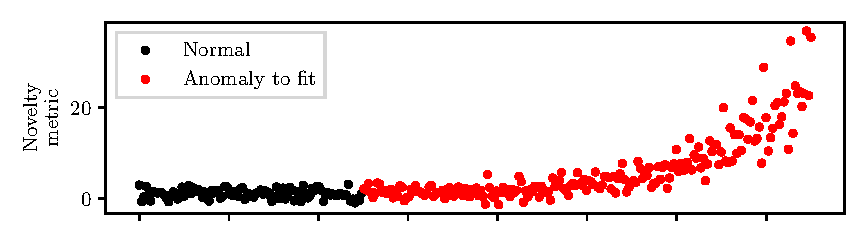
\includegraphics[width=\linewidth]{images/Framework/EXP_1.pdf}
        \caption{}
        \label{fig:exp_degradation_1}
    \end{subfigure}
    \begin{subfigure}{\textwidth}
        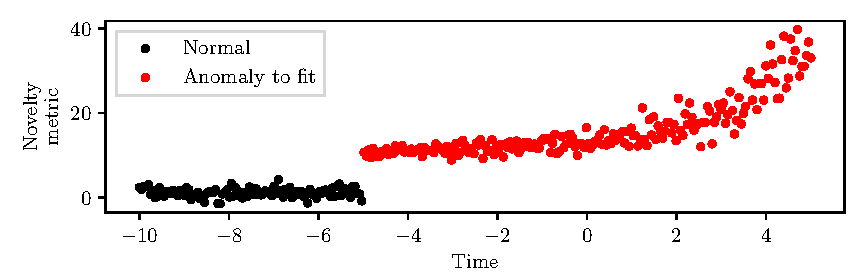
\includegraphics[width=\linewidth]{images/Framework/EXP_2.pdf}
        \caption{}
        \label{fig:exp_degradation_2}
    \end{subfigure}
    \caption{Novelty metric data to fit with an exponential curve.}
    \label{fig:mainfig}
    \label{fig:exp_degradation}
\end{figure}

The metric generated by the \gls{mla} is useful to detect novelties, with a \gls{cbm} approach. To actually perform \gls{pdm}, the \gls{mla} has also to predict the future evolution of the metric. Since, as anticipated in the introduction, this \gls{glo:frmwrk} aims to output \emph{degradation based} predictions, a suitable fitting curve has to be used. Degradation-based failures are led by an initial defect that worsens over time. Often, the presence of an early defect further increases the worsening rate of the system. For this reason, and by observing the \gls{glo:feature}s evolution on publically available datasets, it seems reasonable to model the degradation with an exponential curve. This approach has been used in \cite{exp_degradation} and \cite{exp_degradation_NeuralNN}.

The candidate function to fit would then be:

\begin{equation}
    \label{eq:exp_degradation}
    f(t) = a \cdot e^{b \cdot t}
\end{equation}

where $a$ and $b$ are the parameters to be estimated. This may work in the case depicted in \autoref{fig:exp_degradation_1}, in which the novelty metric starts from zero and then increases exponentially. This is a problem for a general case in which the metric can have a plateau, or start as a step that captures the initial behaviour of the early defect, and then start an exponential decay, as the example in \autoref{fig:exp_degradation_2}. In our case, in \autoref{ch:Unsupervised}, the set of defined metrics to be used are usually negative, to depict a normal behaviour, and not zero. 

The \autoref{eq:exp_degradation} is nice because, by extracting the logarithm from both sides (and calling $y = \log(f(t))$), we obtain a linear equation that can be fitted easily with the least squares method described in \autoref{subsec:LS}. Anyway, for the reasons explained above, it's not suitable for our case. A better candidate is:

\begin{equation}
    \label{eq:exp_degradation_2}
    f(t) = a \cdot e^{b \cdot t} + c
\end{equation}

This is a better candidate because it can depict the case in which the metric starts from a value different from zero, and then increases exponentially.

\subsubsection{\texttt{Scipy} fit}
Unfortunately, \autoref{eq:exp_degradation_2} cannot be arranged in linear form, so the least squares solution has to be found with some other procedure. The \texttt{\gls{glo:python}} library \texttt{scipy.optimize} has a function called \texttt{curve\_fit} that can be used to fit a generic function to a dataset. The problem with this recursive solution is that is very sensitive to outliers and can't really estimate the parameter $c$ correctly, as is shown in \autoref{fig:exp_degradation_3}.

\subsubsection{Closed form fit with least squares}
Fortunately, in \cite{Exp_fit}, the author provides a \emph{nonrecursive} solution to the problem that minimizes the \gls{ls} error \gls{wrt} the parameters $a$, $b$ and $c$. The solution has been converted into the following \autoref{alg:expfit} and implemented in the \gls{glo:frmwrk}. The fitting with this closed-form solution is shown in \autoref{fig:exp_degradation_3}. This optimal solution is used as default in the \gls{glo:frmwrk} to predict the future evolution of the metric, the \texttt{scipy} implementation can still be used by changing a parameter in the configuration file because it has the advantage of fitting any function, so it may be useful in special cases.

\begin{algorithm}
    \caption{Exponential regression of the novelty metric.}
    \label{alg:expfit}
    \begin{algorithmic}[1]
      \Function{ExpRegression}{$x, y$}
      \LineComment{$x = \{x_1, \dots, x_n\}$ is the array of x-coordinates of the data points.}
      \LineComment{$y = \{y_1, \dots, y_n\}$ is the array of y-coordinates of the data points.}
      \LineComment{Returns the parameters $a$, $b$ and $c$ of the exponential function $y(x) = a \cdot e^{b \cdot x} + c$ that minimizes the least squares error.}
      \State $S_1 \gets 0$
      \State $S_k \gets S_{k-1}+\frac{1}{2}(y_k+y_{k-1})(x_k-x_{k-1}) \quad \text{for} \quad k \in [2, n]\cap \mathbb{N}$
      \State $\begin{bmatrix}
        A_1 \\
        B_1        
      \end{bmatrix} \gets \begin{bmatrix}
        \Sigma(x_k-x_1)^2 & \Sigma(x_k-x_1)\cdot S_k \\
        \Sigma(x_k-x_1)\cdot S_k & \Sigma S_k^2        
      \end{bmatrix}^{-1}
      \begin{bmatrix}
        \Sigma(y_k-y_1)(x_k-x_1) \\
        \Sigma(y_k-y_1)\cdot S_k  
      \end{bmatrix}$
      \State $a_1 \gets -\frac{A_1}{B_1}$
        \State $c_1 \gets B_1$
        \State $c_2 \gets c_1$
        \State $\theta_k \gets e^{c_2\cdot x_k} \quad \forall k \in [1, n]\cap \mathbb{N}$
        \State $\begin{bmatrix}
            a_2 \\
            b_2
        \end{bmatrix} \gets 
        \begin{bmatrix}
            n & \Sigma \theta_k \\
            \Sigma \theta_k & \Sigma \theta_k^2
        \end{bmatrix}^{-1}
        \begin{bmatrix}
            \Sigma y_k \\
            \Sigma y_k \cdot \theta_k
        \end{bmatrix}$
        \State $a \gets b_2$
        \State $b \gets c_2$
        \State $c \gets a_2$
        \State \Return $a, b, c$
      \EndFunction
    \end{algorithmic}
  \end{algorithm}
  

\begin{figure}
    \centering
    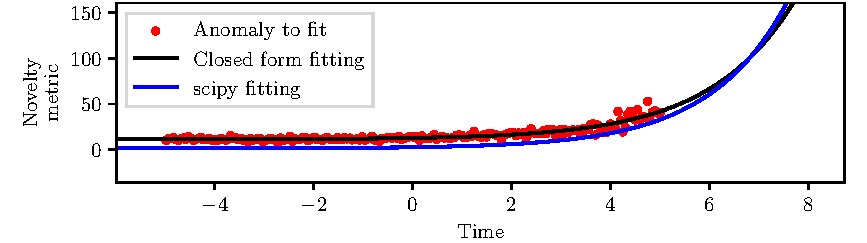
\includegraphics[width=\textwidth]{images/Framework/EXP_3.pdf}
    \caption{Fitted curve for \gls{rul} prediction. The \texttt{scipy} library fit fails to estimate the parameter $c$. The closed-form solution actually minimizes the error.}
    \label{fig:exp_degradation_3}
\end{figure}

\subsection{Instance structure}

\begin{figure}
    \centering
    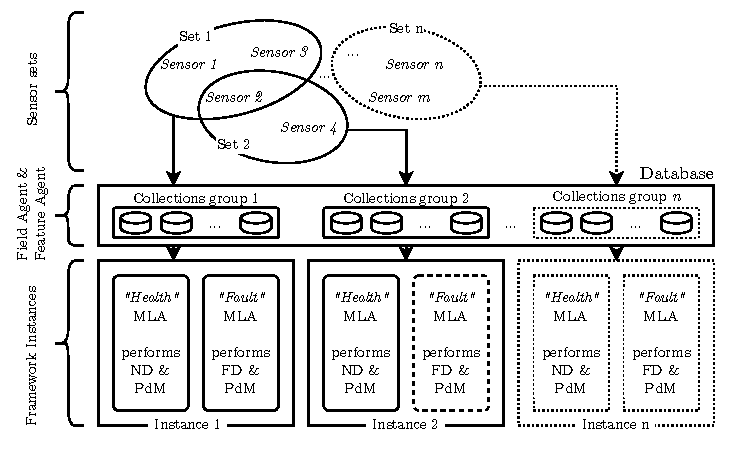
\includegraphics[scale=1]{images/Framework/FrameworkInstances.pdf}
    \caption{The structure of the instances of the \gls{glo:frmwrk}.}
    \label{fig:instance_structure}
\end{figure}

As anticipated, in order to address different kinds of malfunctions, the \gls{glo:frmwrk} is thought to be instanced several times on the same system. To visualize the structure of the instances, consider the general case described in \autoref{fig:instance_structure}. Any instance can rely on data gathered from any sensor subset and can perform \gls{nd} and \gls{fd}. In the figure, the first instance reads the first three sensors and has both the \gls{nd} and \gls{fd} algorithms active (this means that a fault dataset has been gathered in the past). The second instance reads a shared sensor with the first one, plus two new sensors. The dashed line surrounding the \gls{fd} algorithm means that it is not active (no fault dataset has been gathered in the past, or it has not been trained). This instance performs only \gls{nd}. The last instance is just a general prosecution of the structure, that can be scaled indefinitely.
